\documentclass[a4paper,titlepage,11pt,twosides,floatssmall]{mwrep}
\usepackage[left=2.5cm,right=2.5cm,top=2.5cm,bottom=2.5cm]{geometry}
\usepackage[OT1]{fontenc}
\usepackage{polski}
\usepackage{amsmath}
\usepackage{amsfonts}
\usepackage{amssymb}
\usepackage{graphicx}
\usepackage{float}
\usepackage{url}
\usepackage{tikz}
\usetikzlibrary{arrows,calc,decorations.markings,math,arrows.meta}
\usepackage{rotating}
\usepackage[percent]{overpic}
\usepackage[cp1250]{inputenc}
\usepackage{xcolor}
\usepackage{colortbl}
\usepackage{pgfplots}
\usetikzlibrary{pgfplots.groupplots}
\usepackage{listings}
\usepackage{matlab-prettifier}
\usepackage{enumitem,amssymb}
\definecolor{szary}{rgb}{0.95,0.95,0.95}
\usepackage{siunitx}
\usepackage{gensymb} %do st. Celsjusza
\usepackage{graphicx} %do załączania png
\sisetup{detect-weight,exponent-product=\cdot,output-decimal-marker={,},per-mode=symbol,binary-units=true,range-phrase={-},range-units=single}
\SendSettingsToPgf
%konfiguracje pakietu listings
\lstset{
	backgroundcolor=\color{szary},
	frame=single,
	breaklines=true,
}
\lstdefinestyle{customlatex}{
	basicstyle=\footnotesize\ttfamily,
	%basicstyle=\small\ttfamily,
}
\lstdefinestyle{customc}{
	breaklines=true,
	frame=tb,
	language=C,
	xleftmargin=0pt,
	showstringspaces=false,
	basicstyle=\small\ttfamily,
	keywordstyle=\bfseries\color{green!40!black},
	commentstyle=\itshape\color{purple!40!black},
	identifierstyle=\color{blue},
	stringstyle=\color{orange},
}
\lstdefinestyle{custommatlab}{
	captionpos=t,
	breaklines=true,
	frame=tb,
	xleftmargin=0pt,
	language=matlab,
	showstringspaces=false,
	basicstyle=\footnotesize\ttfamily,
	%basicstyle=\scriptsize\ttfamily,
	keywordstyle=\bfseries\color{green!40!black},
	commentstyle=\itshape\color{purple!40!black},
	identifierstyle=\color{blue},
	stringstyle=\color{orange},
}

%wymiar tekstu (bez zywej paginy)
\textwidth 160mm \textheight 247mm

%ustawienia pakietu pgfplots
\pgfplotsset{
tick label style={font=\scriptsize},
label style={font=\small},
legend style={font=\small},
title style={font=\small}
}

\def\figurename{Rys.}
\def\tablename{Tab.}

%konfiguracja liczby plywajacych elementow
\setcounter{topnumber}{0}%2
\setcounter{bottomnumber}{3}%1
\setcounter{totalnumber}{5}%3
\renewcommand{\textfraction}{0.01}%0.2
\renewcommand{\topfraction}{0.95}%0.7
\renewcommand{\bottomfraction}{0.95}%0.3
\renewcommand{\floatpagefraction}{0.35}%0.5

% do tabeli
\usepackage{multirow}


\begin{document}
\frenchspacing
\pagestyle{uheadings}

%strona tytulowa
\title{\bf Sprawozdanie z projektu i �wiczenia laboratoryjnego nr 3, zadanie nr 2\vskip 0.1cm}
\author{Eva Reszka, Mateusz Roszkowski,  Dominika Zaj�c}
\date{2021}

\makeatletter
\renewcommand{\maketitle}{\begin{titlepage}
\begin{center}{\LARGE {\bf
Wydzia� Elektroniki i Technik Informacyjnych}}\\
\vspace{0.4cm}
{\LARGE {\bf Politechnika Warszawska}}\\
\vspace{0.3cm}
\end{center}
\vspace{5cm}
\begin{center}
{\bf \LARGE Projektowanie uk�ad�w sterowania\\ (projekt grupowy) \vskip 0.1cm}
\end{center}
\vspace{1cm}
\begin{center}
{\bf \LARGE \@title}
\end{center}
\vspace{2cm}
\begin{center}
{\bf \Large \@author \par}
\end{center}
\vspace*{\stretch{6}}
\begin{center}
\bf{\large{Warszawa, \@date\vskip 0.1cm}}
\end{center}
\end{titlepage}
}
\makeatother

\maketitle

\tableofcontents
% !TEX encoding = cp1250
\chapter{Projekt}



\section{Sprawdzenie poprawno�ci punktu pracy}

Implementacja zadania znajduje si� w pliku \texttt{zad1\_2.m}.

Punkt pracy r�wny jest $U_{pp} = 0$, $Y_{pp} = 0$, co zosta�o przedstawione na wykresach \ref{zad1_u} i \ref{zad1_y}.

\begin{figure}[H]
	\centering
	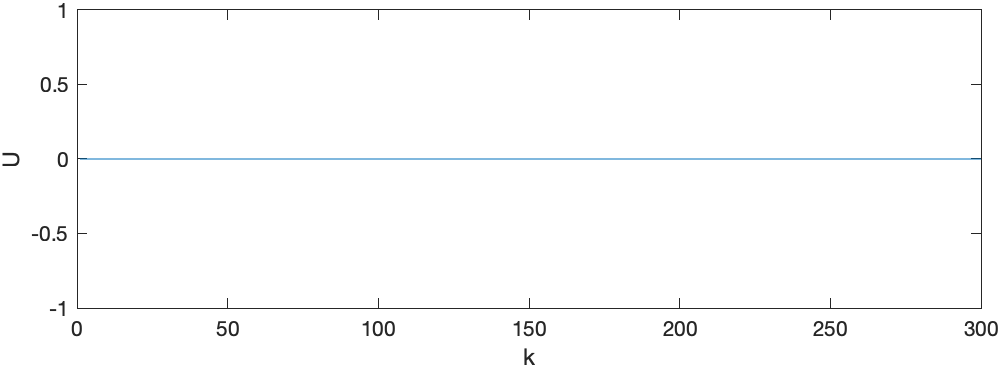
\includegraphics[scale=0.75]{png/projekt/zad1_u.png}
	\caption{Wej�cie uk�adu w punkcie pracy}
	\label{zad1_u}
\end{figure}

\begin{figure}[H]
	\centering
	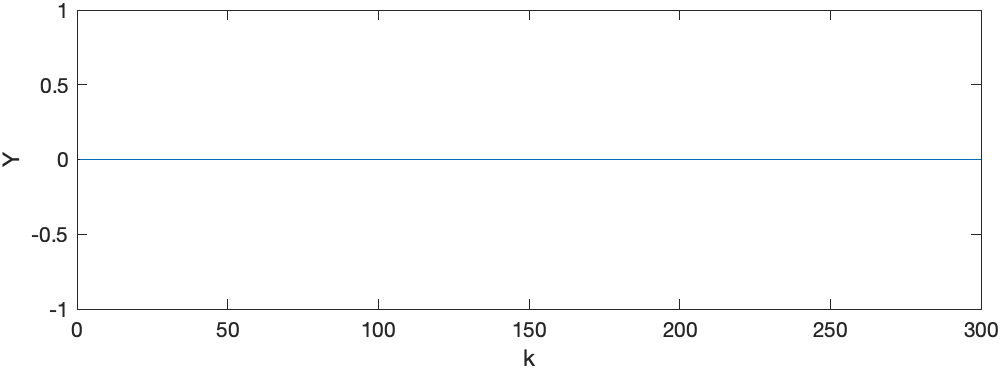
\includegraphics[scale=0.75]{png/projekt/zad1_y.png}
	\caption{Wyj�cie uk�adu w punkcie pracy}
	\label{zad1_y}
\end{figure}

 
\section{Wyznaczenie odpowiedzi skokowych procesu}

Uk�ad zosta� pobudzony sygna�ami o warto�ciach $ U = [-0,8; -0,3; 0,2; 0,6; 1,0]$.

Otrzymane zosta�y w ten spos�b odpowiedzi skokowe:

\begin{figure}[H]
	\centering
	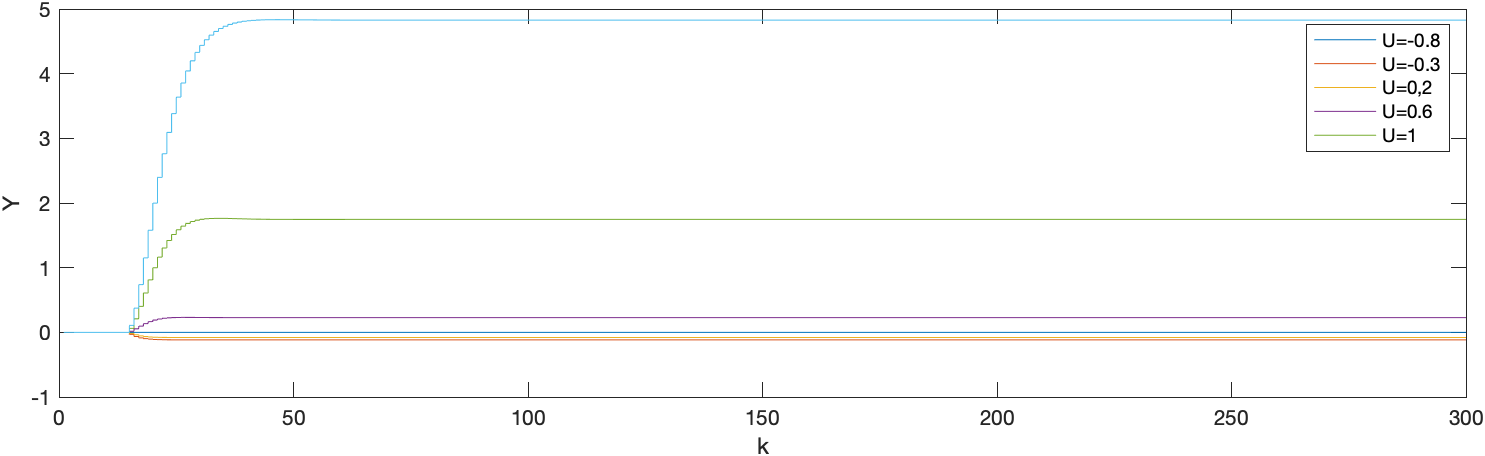
\includegraphics[scale=0.6]{png/projekt/zad2_1.png}
	\caption{Otrzymane odpowiedzi skokowe}
	\label{zad2_1}
\end{figure}

Na wykresie  \ref{zad2_2}  widoczna jest charakterystyka statyczna obiektu.

\begin{figure}[H]
	\centering
	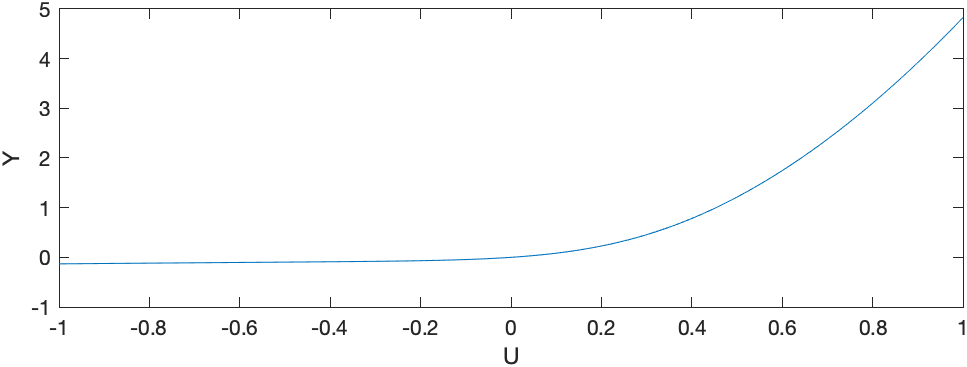
\includegraphics[scale=0.75]{png/projekt/zad2_2.png}
	\caption{Charakterystyka statyczna}
	\label{zad2_2}
\end{figure}

W�a�ciwo�ci dynamiczne oraz statyczne nie s� liniowe. Do charakterystyki statycznej nie mo�e zosta� dopasowana prosta.

\section{Algorytmy PID i DMC}

Obiekt zosta� poddany regulacji za pomoc� algorytm�w PID i DMC z Projektu 2.

TODO opis PID, DMC

\begin{figure}[H]
	\centering
	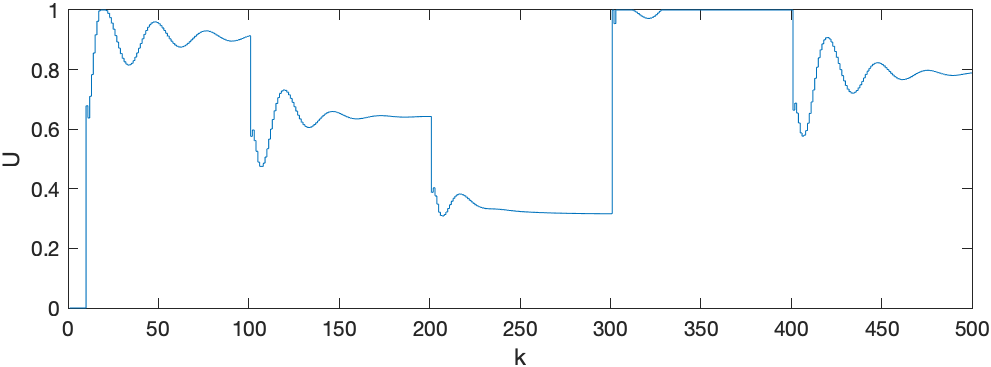
\includegraphics[scale=0.75]{png/projekt/zad3_pid_u.png}
	\caption{Wej�cie uk�adu - algorytm PID}
	\label{zad3_pid_u}
\end{figure}

\begin{figure}[H]
	\centering
	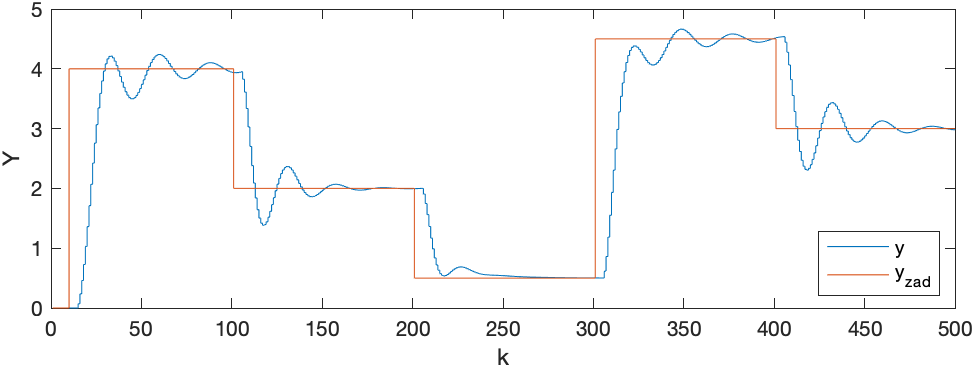
\includegraphics[scale=0.75]{png/projekt/zad3_pid_y.png}
	\caption{Wyj�cie uk�adu - algorytm PID}
	\label{zad3_pid_y}
\end{figure}

\begin{figure}[H]
	\centering
	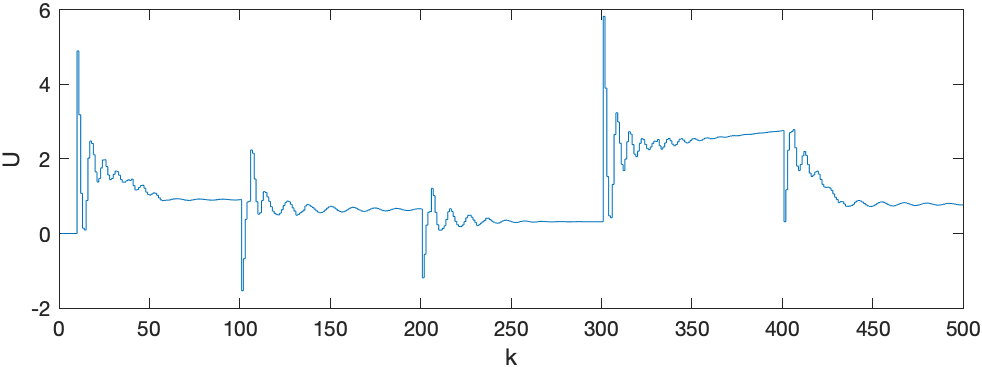
\includegraphics[scale=0.75]{png/projekt/zad3_dmc_u.png}
	\caption{Wej�cie uk�adu - algorytm PID}
	\label{zad3_dmc_u}
\end{figure}

\begin{figure}[H]
	\centering
	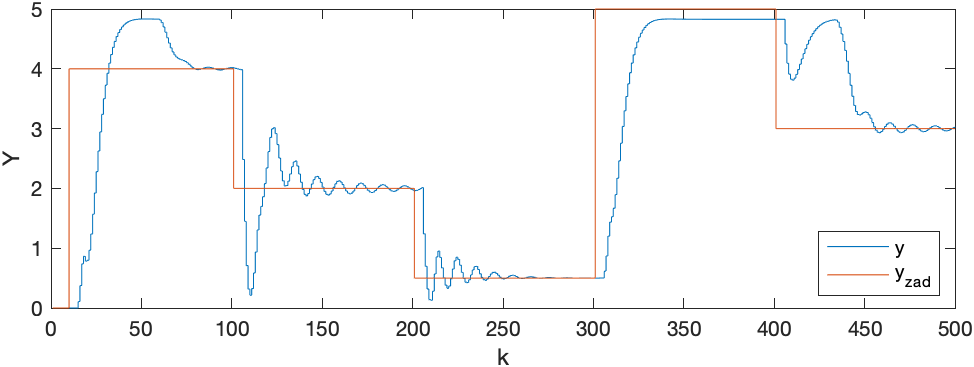
\includegraphics[scale=0.75]{png/projekt/zad3_dmc_y.png}
	\caption{Wyj�cie uk�adu - algorytm PID}
	\label{zad3_dmc_y}
\end{figure}



\section{Rozmyty algorytm PID}

\section{Rozmyty algorytm DMC}


% !TEX encoding = cp1250
\chapter{�wiczenie laboratoryjne}

Podczas tego zadania laboratoryjnego wykorzystano:
\begin{itemize}
	\item grza�k� G1 (sygna� steruj�cy $U$),
	\item wentylator W1 (warto�� zadana $Y_{zad}$),
	\item czujnik temperatury T1 (sygna� wyj�ciowy $Y$) 
\end{itemize} 

\section{Przygotowanie do wykonania �wiczenia}
Przed rozpocz�ciem pomiar�w sprawdzono mo�liwo�� sterowania i~pomiaru w~komunikacji ze stanowiskiem. Punkt pracy grza�ki $G1$ dla zespo�u obliczony zosta� wg. wzoru \ref{w_G1}:
\begin{equation}
	G1 = 25 + Z\%5\
\label{w_G1}
\end{equation}
gdzie Z~to numer zespo�u, zatem dla naszego zespo�u Z02 punkt pracy wynosi:
\begin{equation}
	G1 = 25 + 2\%5 = 27
\end{equation}
Nast�pnie okre�lono warto�� pomiaru temperatury T1 dla obliczonego punktu pracy. W~tym celu moc wentylatora W1 ustawiono na 50\%, a moc grza�ki G1 na 27\%,  za pomoc� funkcji
\texttt{sendControls([1,5], [50,27])}.
Warto�� pomiaru temperatury odczytano korzystaj�c z~funkcji 
\texttt{readMeasurements(1)}.
Temperatura T1 ustabilizowa�a si� na warto�ci \textbf{32.25\degree C}

 
\section{Wyznaczenie odpowiedzi skokowych procesu}
Zarejestrowano przebieg temperatury T1 dla trzech r�nych zmian sygna�u steruj�cego G1 rozpoczynaj�c z~punktu pracy (27\%) do 10\%, 35\% i~50\%.
Otrzymane przebiegi zmian przedstawiono na Rys. \ref{rys_przebiegi_T1}. 

\textcolor{red}{
	Czy w�a�ciwo�ci statyczne obiektu mo�na okre�li� jako (w przybli�eniu) liniowe? Je�li tak wyznaczy� wzmocnienie statyczne procesu?
}

\newpage
\begin{figure}[H]
	\centering
	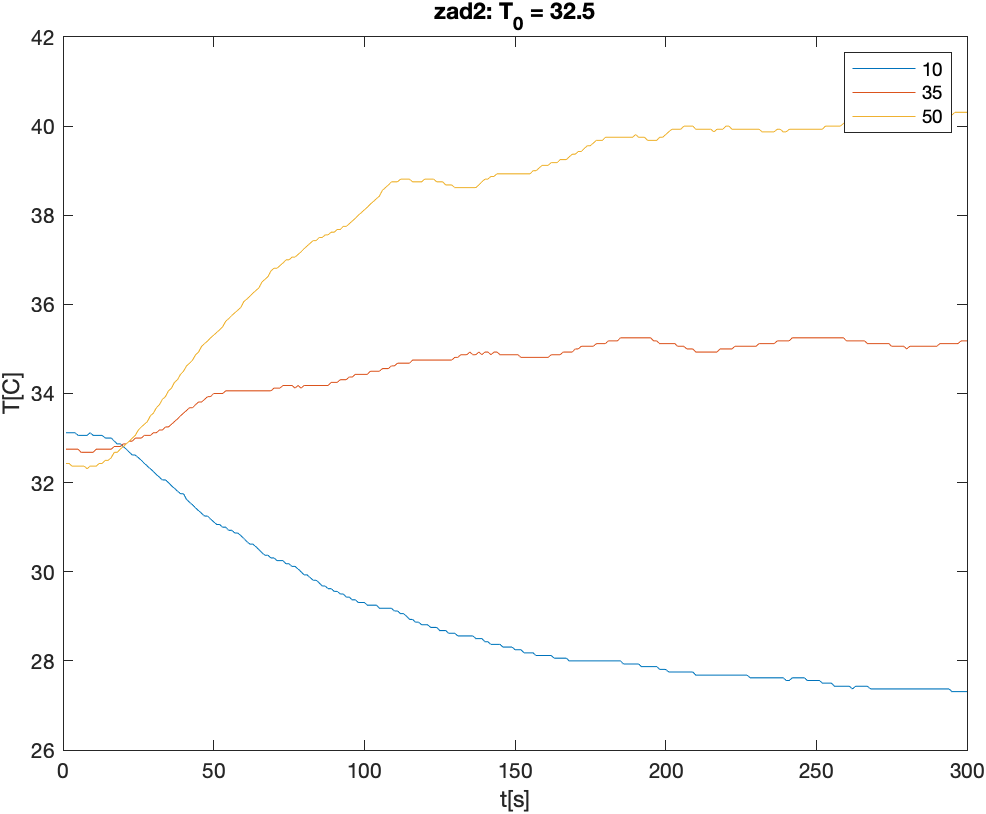
\includegraphics[scale=0.35]{png/lab1_zad2.png}
	\caption{Odpowiedzi skokowe procesu}
	\label{rys_przebiegi_T1}
\end{figure}

\section{Algorytm PID}

Poni�sze zadanie laboratoryjne realizowane by�o w inny, zimniejszy dzie�, co spowodowa�o konieczno�� wyznaczenia warto�ci pomiaru temperatury w punkcie pracy na nowo. Nowy punkt pracy dla ${G1 = 27}$ to ${ T1 = 29.37 }$ {\degree C}.

Napisano  program do regulacji cyfrowego algorytmu PID. Dob�r nastaw regulatora przeprowadzono metod� Zieglera-Nicholsa. Rozpocz�to od doboru warto�ci wzmocnienia K, przy parametrze ca�kuj�cym Ti = inf i r�niczkuj�cym Td = 0. W algorytmie uwzgl�dniono ograniczenia warto�ci sterowania G1(k) (zakres od ${U_{min} = 0}$  do ${\Delta U_{max}=100}$).

Testowano odpowied� uk�adu przy r�nych warto�ciach wzmocnienia K. 
Pocz�tkowo ustawiono zbyt du�� warto�� ${Y_{zad} = 50}$, co uniemo�liwi�o analiz� przebiegu wyj�cia uk�adu � warto�� wzrasta�a powoli, przez co pomiar zajmowa� za du�o czasu. Problem ten widoczny jest na wykresach Rys. {\ref{rys_lab_PID_k18}} i Rys.  {\ref{rys_lab_PID_k20_1}} . Pomiar z Rys. {\ref{rys_lab_PID_k18}} zosta� przerwany po zauwa�eniu nieprzewidywanego zachowania.


\begin{figure}[H]
	\centering
	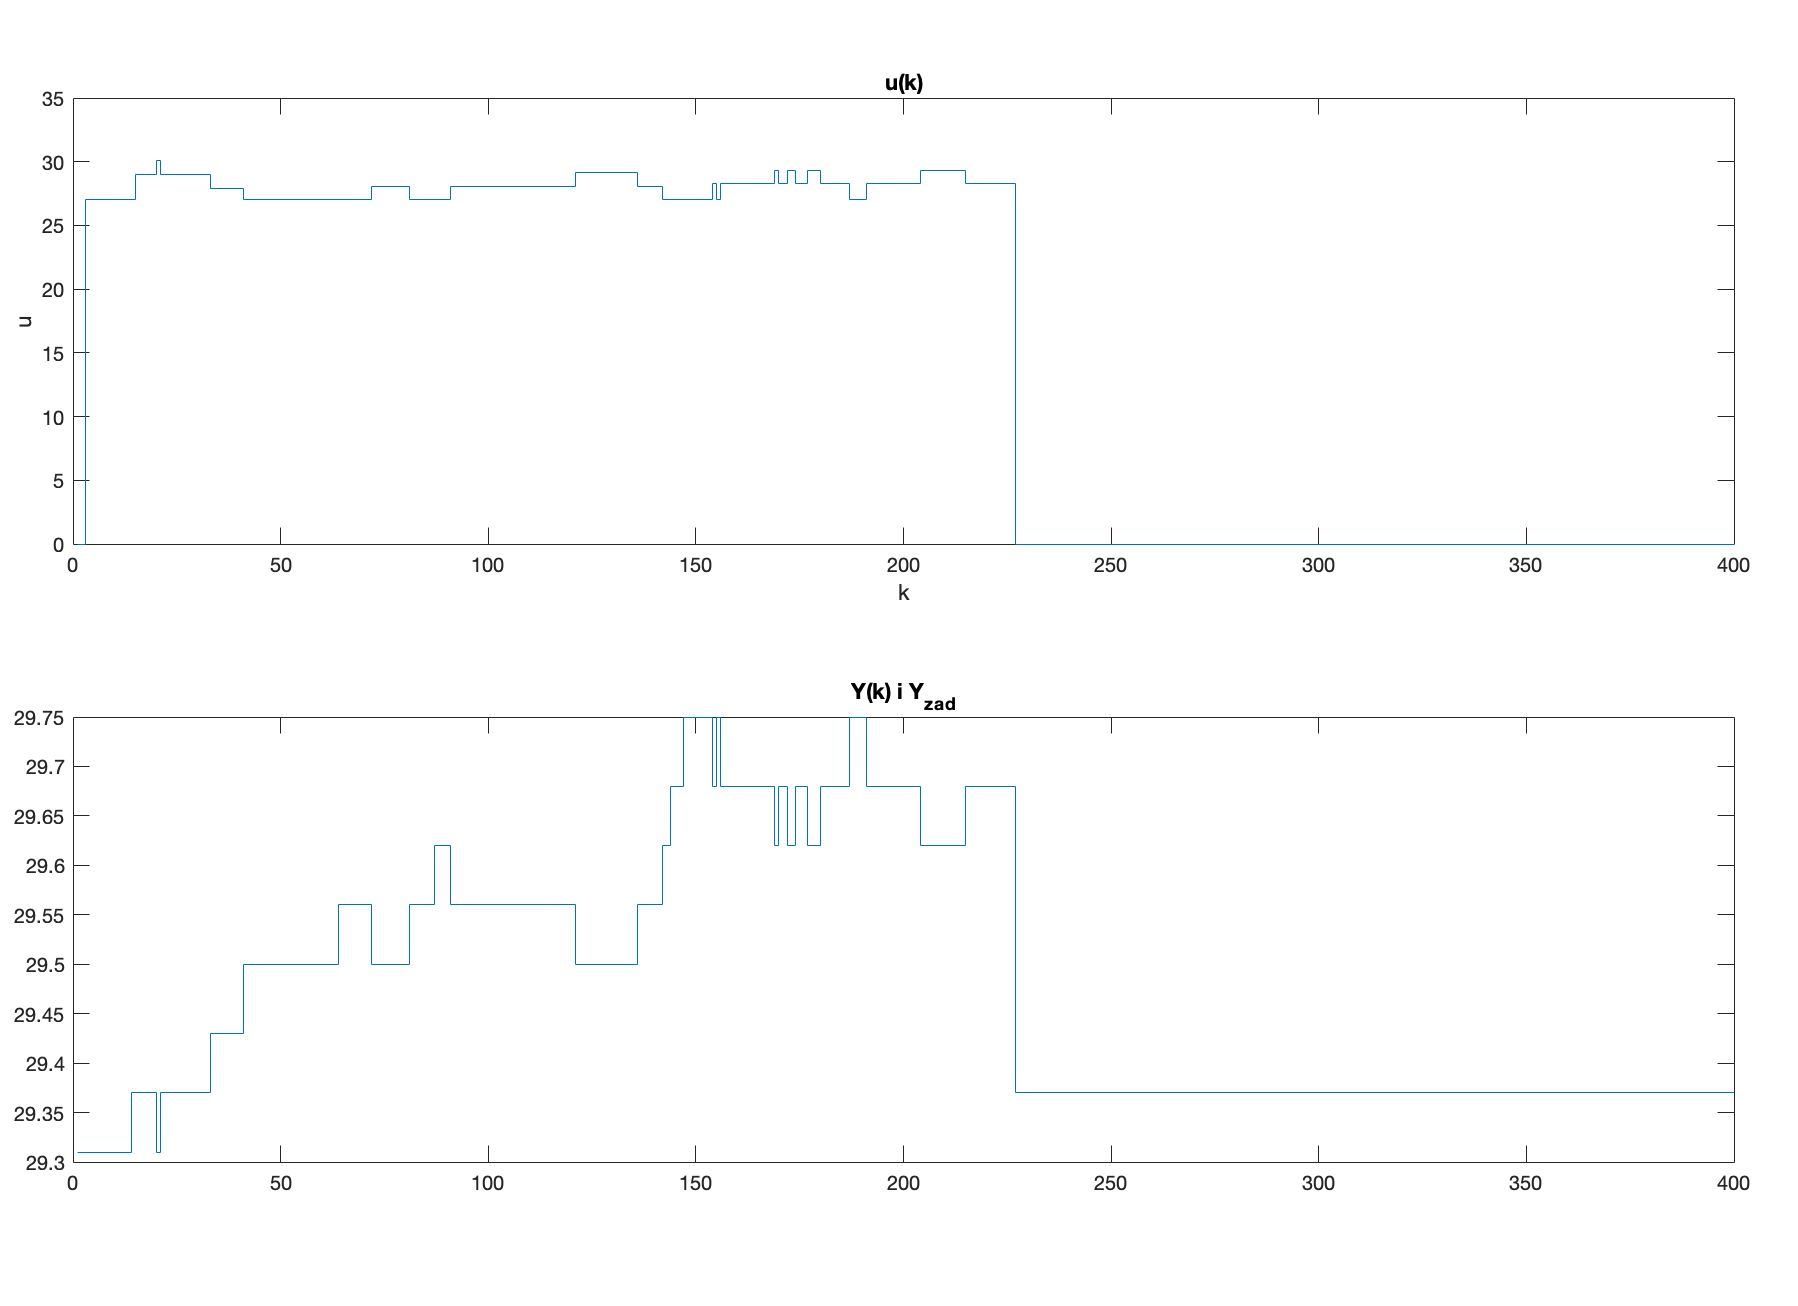
\includegraphics[scale=0.22]{png/lab2/zad5_lab1_pid_k18.png}
	\caption{Przebiegi dla ${K = 18}$ i ${Y_{zad} = 50}$}
	\label{rys_lab_PID_k18}
\end{figure}


\begin{figure}[H]
	\centering
	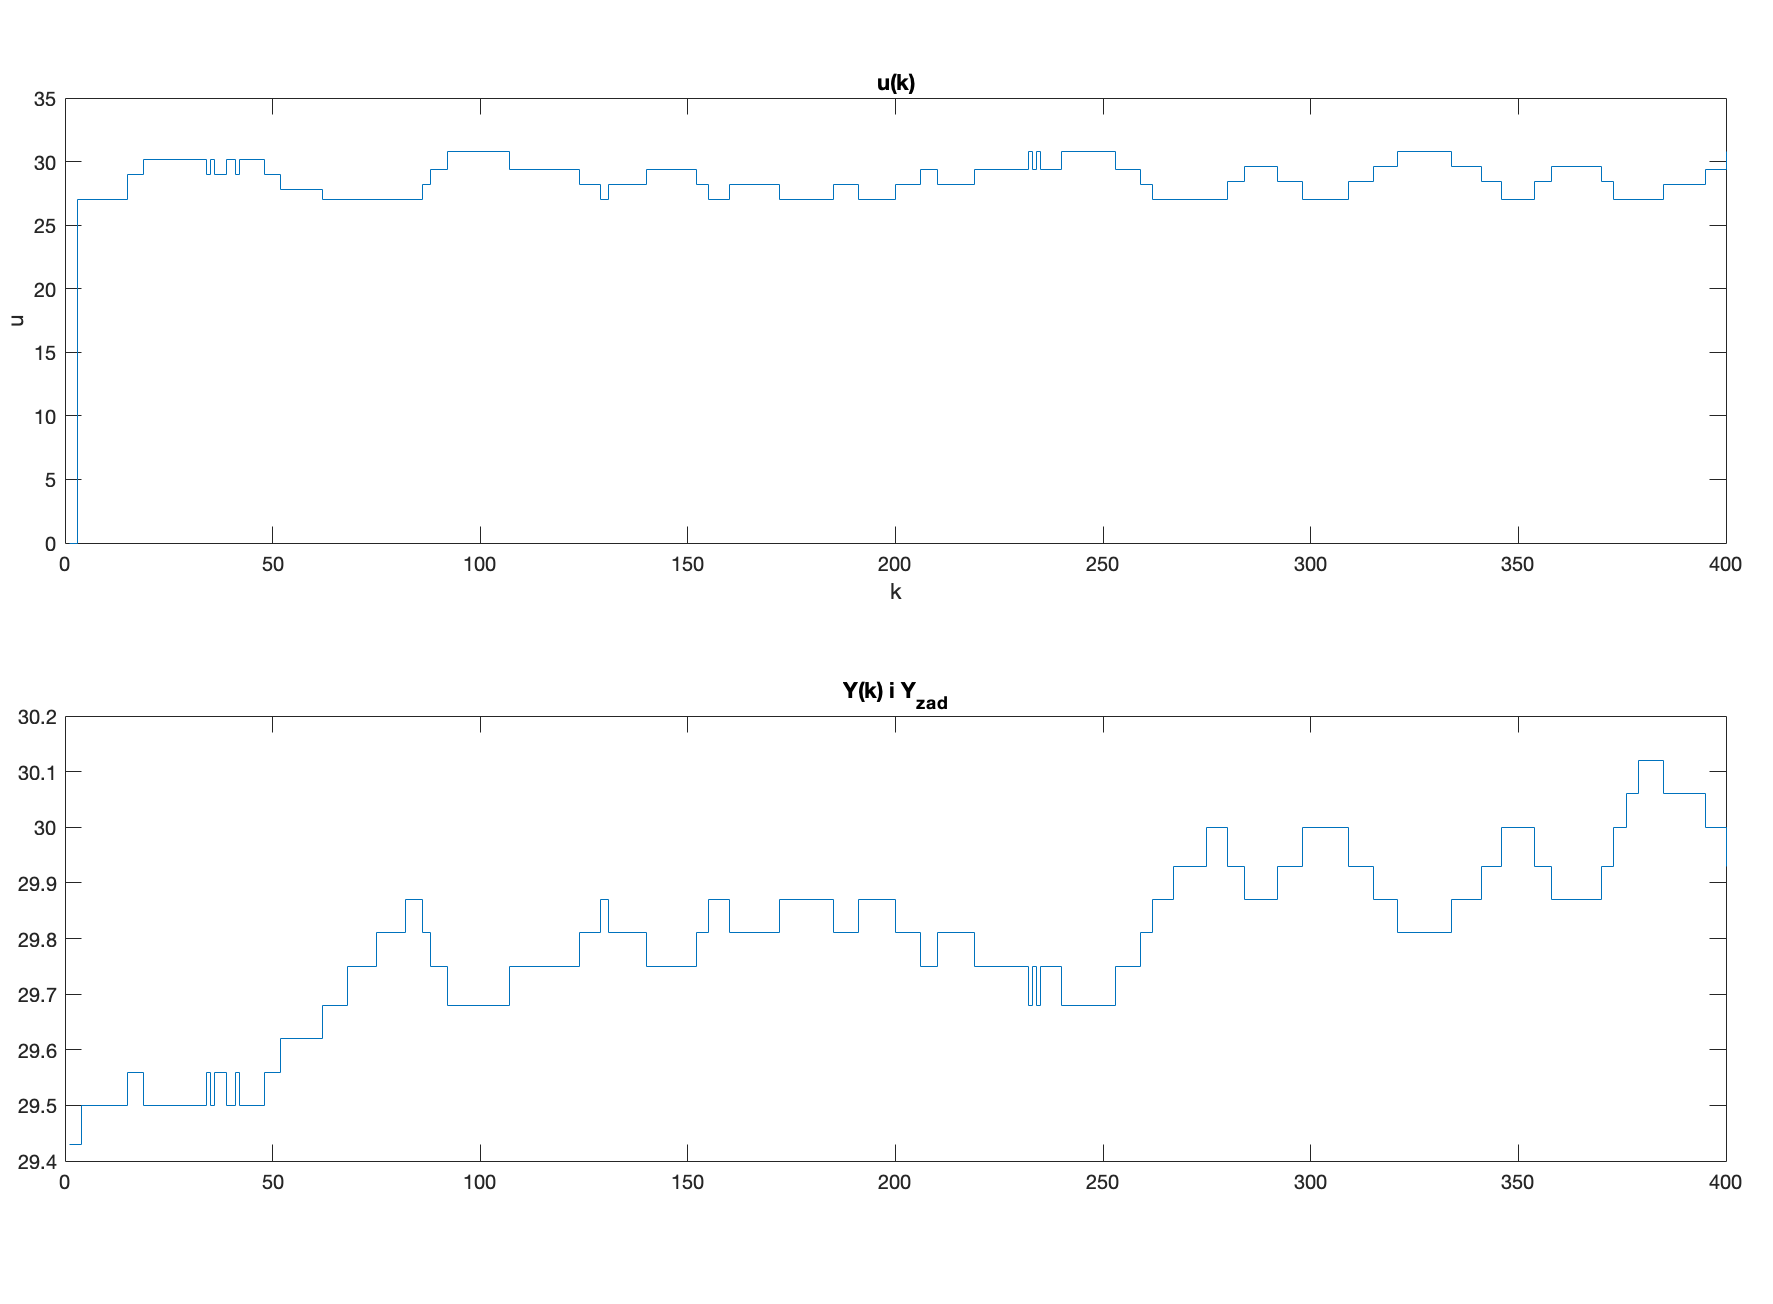
\includegraphics[scale=0.22]{png/lab2/zad5_lab1_pid_k20_v1.png}
	\caption{Przebiegi dla ${K = 20}$ i ${Y_{zad} = 50}$}
	\label{rys_lab_PID_k20_1}
\end{figure}


Po zaobserwowaniu powy�szego problemu i jego analizie zmieniono warto�� sygna�u zadanego na ${Y_{zad} = 33}$. Wyniki widoczne s� na wykresie Rys.  {\ref{rys_lab_PID_k20_2}}.


\begin{figure}[H]
	\centering
	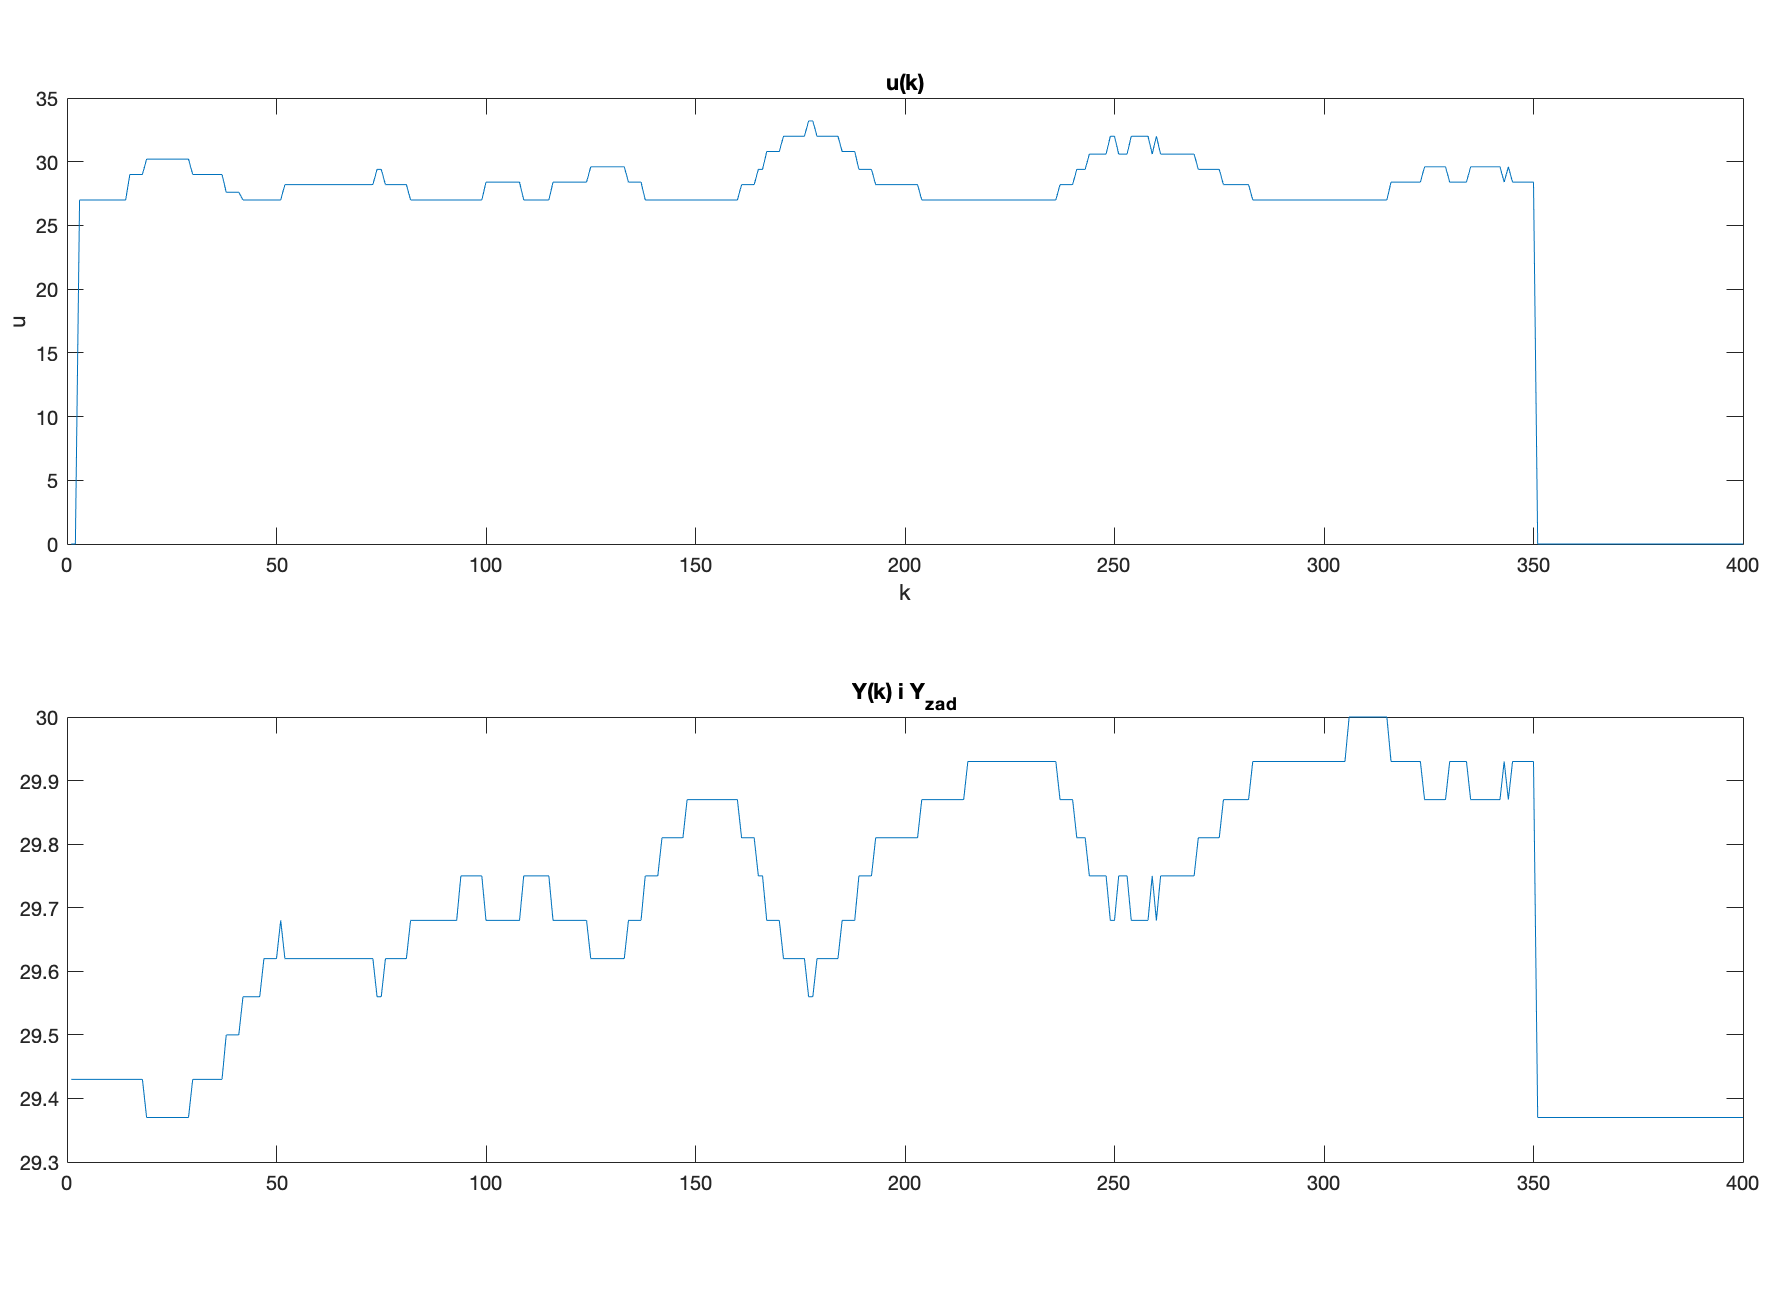
\includegraphics[scale=0.22]{png/lab2/zad5_lab1_pid_k20_v2.png}
	\caption{Przebiegi dla ${K = 20}$ i ${Y_{zad} = 33}$}
	\label{rys_lab_PID_k20_2}
\end{figure}

Mimo tej zmiany, odpowied� procesu nadal ros�a zbyt wolno. Po ponownej analizie algorytmu wywnioskowano, �e do niskiej pr�dko�ci wzrastania przyczyni� si� r�wnie� niew�a�ciwie dobrany parametr ${\Delta U_{max}=2}$ � ogranicza� on bowiem szybko�� zmian sygna�u steruj�cego. Po zmianie tej warto�ci na ${\Delta U_{max} = 20}$, uk�ad dzia�a� zgodnie z za�o�eniami (Rys. {\ref{rys_lab_PID_k20_3}}). 


\begin{figure}[H]
	\centering
	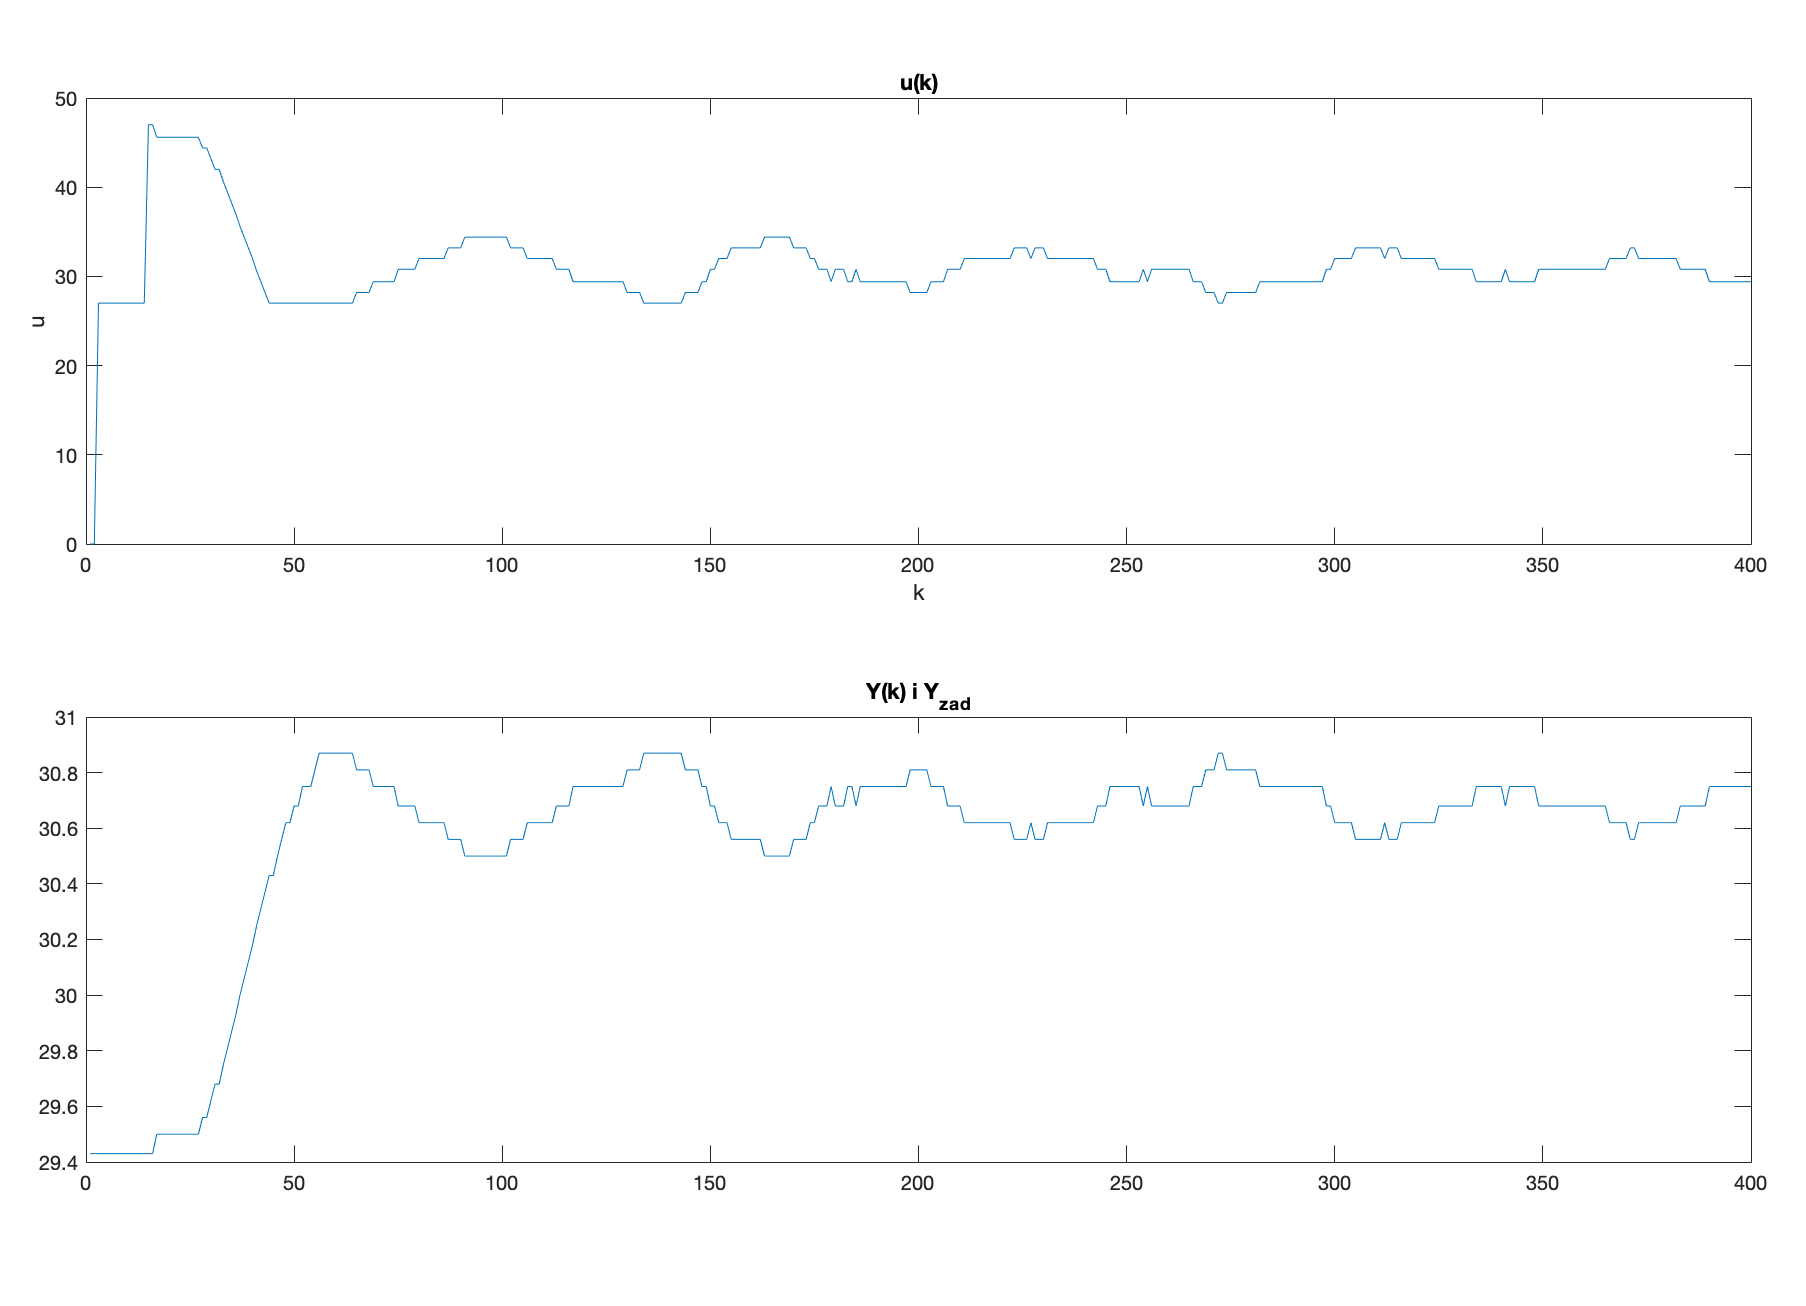
\includegraphics[scale=0.22]{png/lab2/zad5_lab1_pid_k20_v3.png}
	\caption{Przebiegi dla ${K = 20}$, ${Y_{zad} = 33}$ i zmienion� warto�ci� ${\Delta U_{max}}$}
	\label{rys_lab_PID_k20_3}
\end{figure}

Widoczne s� regularne oscylacje, jednak s� one oscylacjami gasn�cymi. Warto�� wzmocnienia zosta�a wi�c zwi�kszona do ${K = 24}$. Jak wida� na wykresie Rys. {\ref{rys_lab_PID_k24}} oscylacje nie gasn�. Zauwa�alny jest  nawet lekki wzrost amplitudy oscylacji. Przewidujemy, �e niegasn�ce oscylacje wyst�pi�yby przy warto�ci wzmocnienia ${K_{kr}=23}$, jednak przez problemy wyst�puj�ce na pocz�tku realizacji zadania nie zosta�o to sprawdzone.
Z tego powodu nie dobrano r�wnie� pozosta�ych parametr�w regulatora PID dla zmiennego sygna�u zadanego. 
Je�li zesp� mia�by wi�cej czasu, nast�pnym krokiem by�oby ustawienie nastaw regulatora wg. regu� Zieglera-Nicholsa (Rys. {\ref{t_ZN}}). Zatem po wyznaczeniu wzmocnienia krytycznego ${K_{kr}}$, z przebiegu warto�ci sterowania odczytany zosta�by okres krytyczny ${T_{kr}}$, a wst�pne nastawy regulatora PID wynosi�yby: ${K=0.6K_{kr}}$, ${T_i= 0.5T_{kr}}$ i ${T_d=0.125K_{kr}}$. Je�eli by�oby to konieczne, regulator zosta�by dostrojony metod� eksperymentaln�.


\begin{figure}[H]
	\centering
	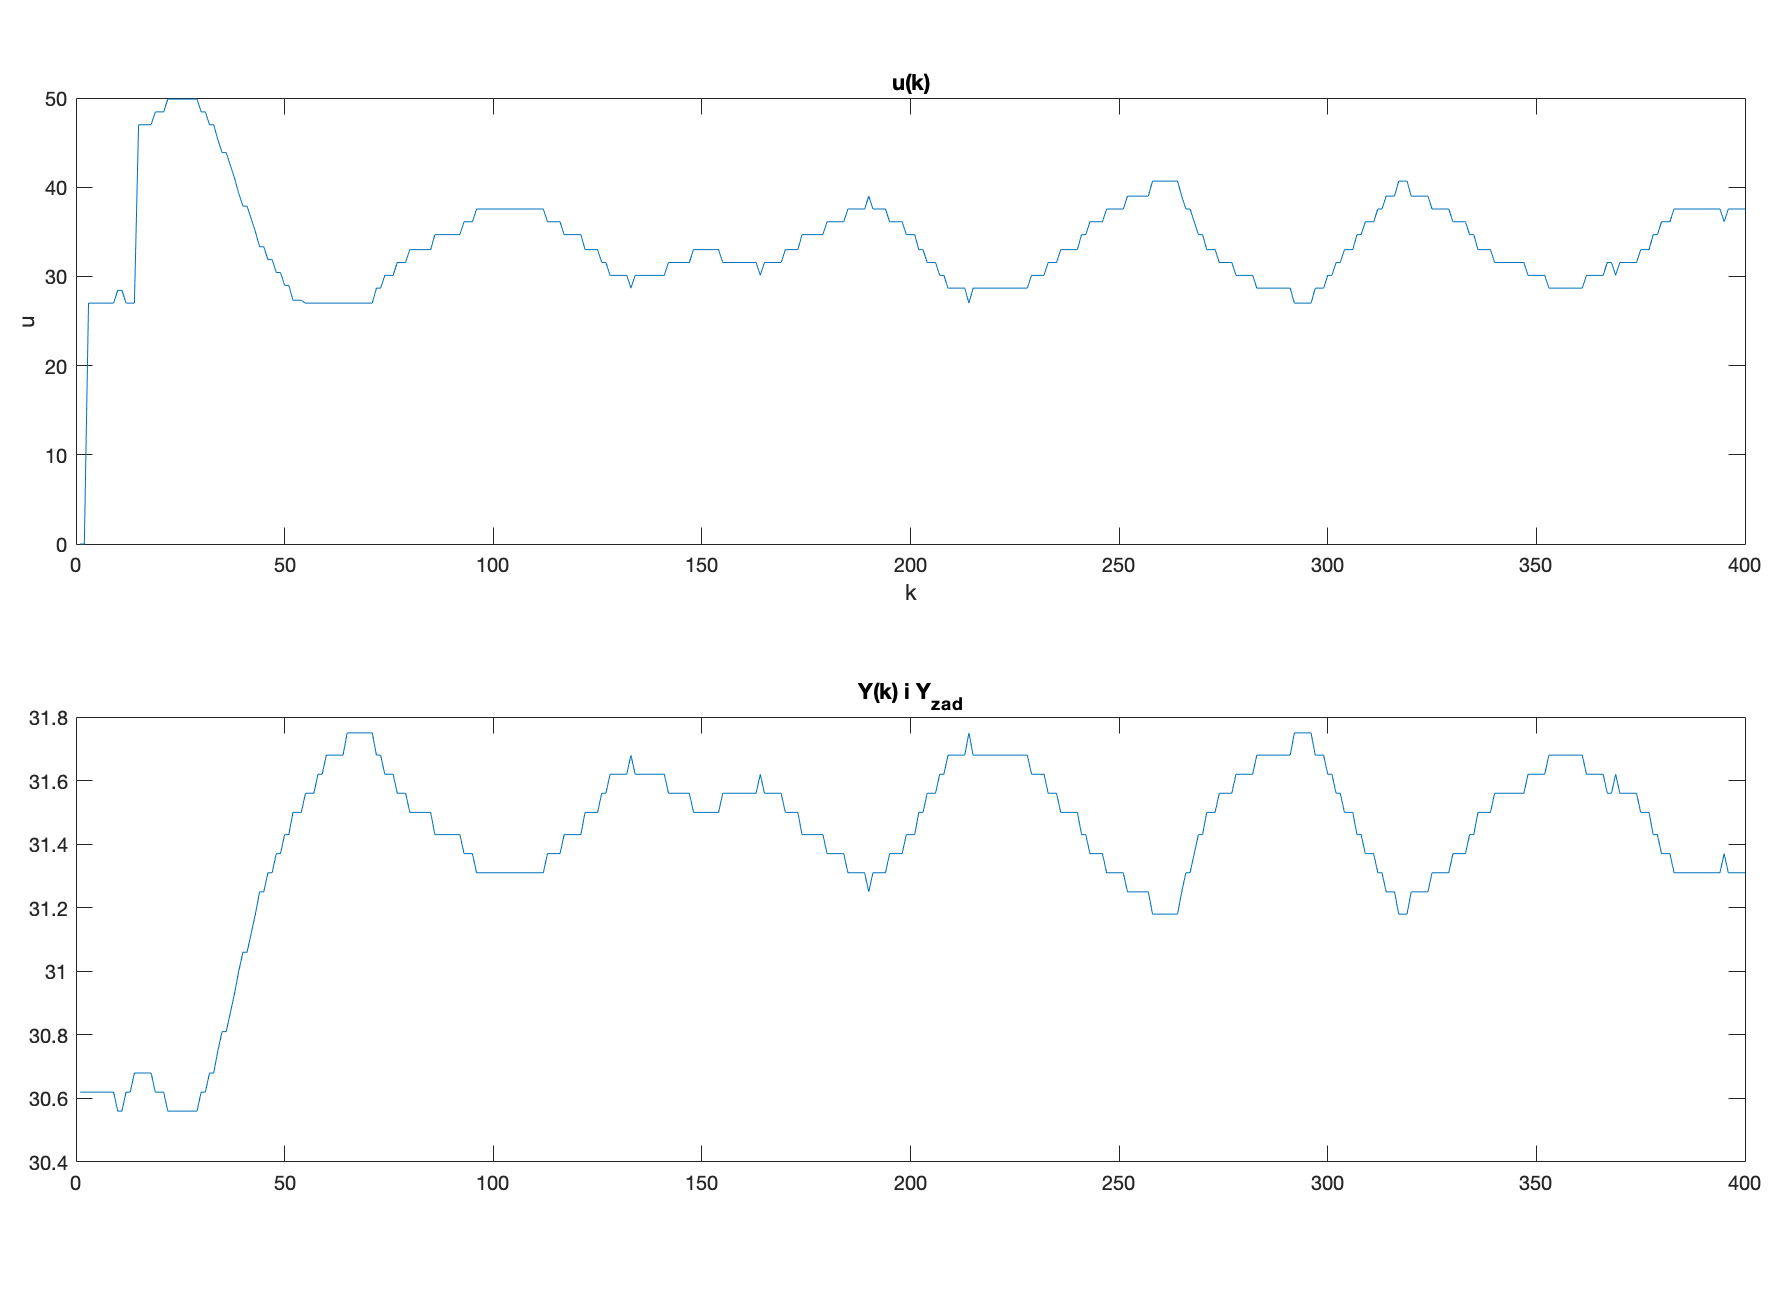
\includegraphics[scale=0.22]{png/lab2/zad5_lab1_pid_k24.png}
	\caption{Przebiegi dla ${K=24}$}
	\label{rys_lab_PID_k24}
\end{figure}



\section{Algorytm DMC}





\end{document}

